\chapter{Demo-Anwendung im Browser}

\section{Anforderungen and die Web-Anwendung}

Um die praktische Anwendung von MiniJava für typische Browser-Anwendungen zu demonstrieren, wurde eine einfache Web-Anwendung implementiert, die Fibonacci-Zahlen berechnen kann. Die Oberfläche soll zwei Eingabefelder (für Werte $a$ und $b$) und einen Start-Knopf darstellen. Beim Drücken des Starknopfs soll die Anwendung die Fibonacci-Zahlen von $fib(a)$ bis $fib(b)$ berechnen und in einer Tabelle darstellen.

Der Fokus der MiniJava-Implementierung ist, MiniJava in einem abgschlossenen Projekt zu präsentieren und zu zeigen, wie MiniJava mit dem Browser interagieren kann. Dabei wurde der Aspekt einer effizienten Implementierung bewusst vernachlässigt. Dadurch wirken zwar einige Code-Abschnitte sehr erzwungen, gleichzeitig wird aber dadurch ermöglicht, im Rahmen eines überschaubaren Anwendungsfalls möglichst viele Features von MiniJava einzusetzen. 

Zum Vergleich wurden diesselben Anforderungen zur Gänze in JavaScript implementiert. Ziel ist lediglich ein einfacher Vergleich zwischen den Programmiersprachen und nicht eine idente oder deckungsgleiche Implementierung.

In diesem Kapitel werden nur relevante Code-Ausschnitte gezeigt, zum Teil wurden einzige Code-Stücke gekürzt. Die vollständige Implementierung findet sich im Git-Re\-pository.

Die Webanwendung wurde auf der folgenden Sofware- und Hardware-Konfigurationg getestet:
\begin{itemize}
    \item Betriebssystem: macOS 10.15.4
    \item Browser: Google Chrome (Mac) 81.0.4044.122 64-Bit
    \item Hardware: MacBook Pro (15-inch, 2018)
    \begin{itemize}
        \item CPU: 2,6 GHz 6-Core Intel Core i7
        \item RAM: 16 GB 2400 MHz DDR4
    \end{itemize}
\end{itemize}

\section{Implementierung in JavaScript}

\lstinputlisting{src/demoAnwendung/js-version.js}

\section{Implementierung in MiniJava}

\lstinputlisting{src/demoAnwendung/ClickEventListener.minijava}
\lstinputlisting{src/demoAnwendung/FibonacciCalculator.minijava}
\lstinputlisting{src/demoAnwendung/Main.minijava}

\section{Build-Prozess und Ausführen der Web-Anwendung}

Ähnlich wie in der Konsolenanwendung im vorherigen Kapitel wird hier ebenfalls Gradle eingesetzt, um den MiniJava-Sourcecode zu kompilieren. Zusätzlich dazu wird webpack \cite{Webpack} eingesetzt, um alle JavaScript-Dateien in eine einzige JavaScript-Datei zusammenzufassen. Sämtliche \lstinline{require}-Referenzierungen werden dabei aufgelöst.

Zusätzlich zur Basis-Standardbibliothek wird eine eigene für den Browser mitkompiliert. Diese enthält Funktionalitäten, die auf Browser-Schnittstellen abgebildet werden (Implementierungdetails sind im nächsten Abschnitt zu finden).

Beim Ausführen muss sichergestellt werden, dass das binäre WebAssembly-Modul vom Web-Server mit dem MIME-Type \lstinline{application/wasm} bereitgestellt wird, sonst kann es zu Laufzeitfehlern kommen \cite{MDNWebAssembly}. Zu Testzwecken reicht dafür das NPM-Modul \lstinline{lite-server}\footnote{\url{https://www.npmjs.com/package/lite-server}} vollkommen aus. Für produktiven Einsatz sollte man diesen Aspekt bei der Konfiguration des Web-Servers beachten.

\section{Auszug aus der Standardbibliothek für den Browser}

Um mit MiniJava sinnvoll mit der Browser interagieren zu können, wurde eine kleine Standardbibliothek dafür entwickelt. Zwei Funktion daraus werden nun im Detail betrachtet: Das Abfragen eines HTML-Knotens aus dem DOM über die ID des Elements und das Hinzufügen eines Event-Listeners für das Maus-Klick-Ereignis zu einem HTML-Knoten.

\lstinputlisting{src/demoAnwendung/Browser.minijava}
\lstinputlisting{src/demoAnwendung/Browser.js}

Nachfolgend einige Details zum JavaScript-Teil der beiden Methoden:

Mit der Funktion \lstinline{runtime.wasmRef} können DOM-Knoten, die die JavaScript-Funktion \lstinline{document.getElementById} zurückgibt, MiniJava zugänglich gemacht werden.

Beim Registrieren des Event-Listeners wird eine JavaScript-Funktion (Lambda-Aus\-druck) registriert. Diese Funktion delegiert das Ereignis an das beim Registieren übergebene \lstinline{handler}-Objekt. Dabei wird angenommen, dass in der Klasse dieses Objekts eine Methode names \lstinline{handleEvent} existiert, die einen Parameter vom Typ \lstinline{MouseEvent} annimmt. Sollte so eine Methode nicht existieren, kommt es zu einem Laufzeitfehler.

\section{Ergebnis}

Nachfolgend sind zwei Screenshots der Fibonacci-Web-Anwendung im Browser. Links wurde die JavaScript-Version ausgeführt, rechts die MiniJava-Version. Man erkennt bei den ersten Zahlen, dass diese korrekt berechnet wurden.

\begin{center}
    \begin{tabular}{c c}
        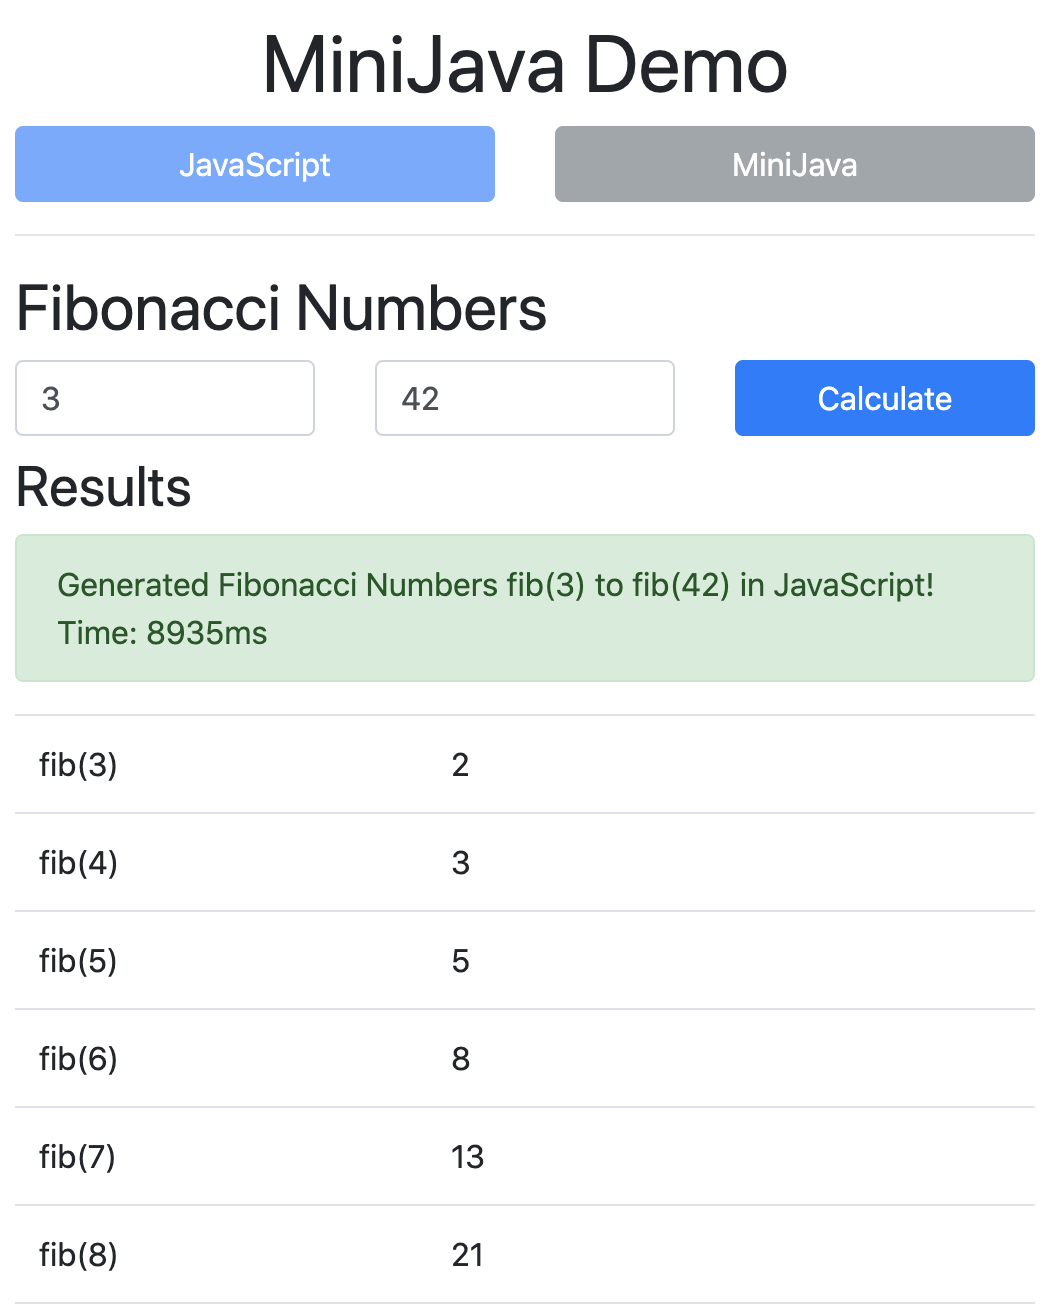
\includegraphics[width=0.47\textwidth]{demoAnwendung/fibonacciJavaScript} & 
        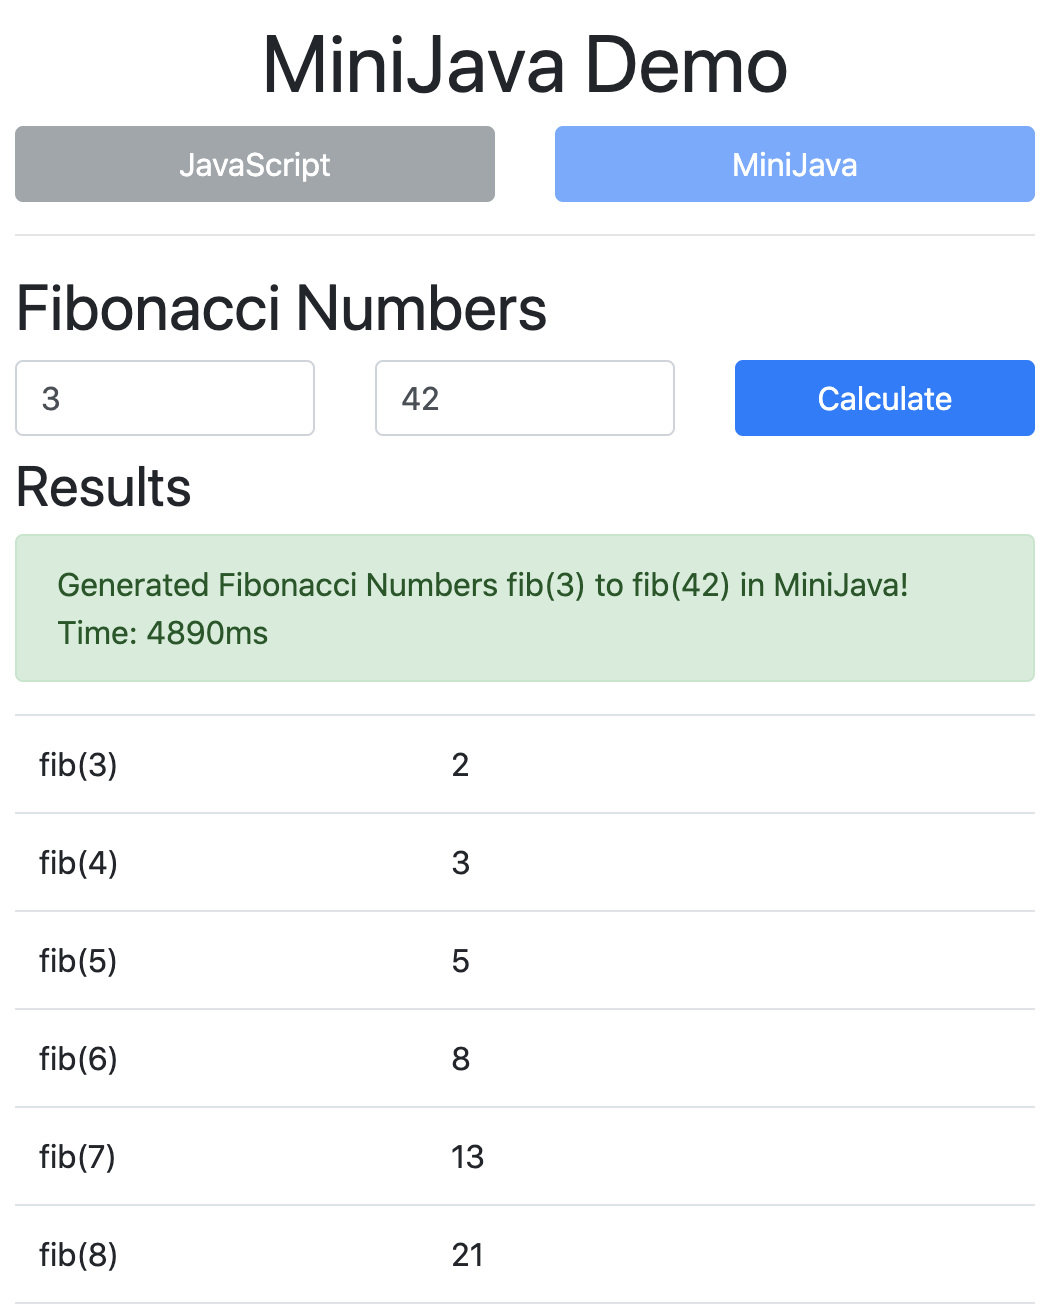
\includegraphics[width=0.47\textwidth]{demoAnwendung/fibonacciMiniJava}
    \end{tabular}
\end{center}

Während dem Ausführen wurde die Laufzeit gemessen, dabei wird die gesamte Zeit ab Klicken des Start-Knopfs bis zum Erstellen der Tabelle berücksichtigt. Man erkennt, dass die Laufzeit der MiniJava-Version (5435 Millisekunden) im Vergleich zur JavaScript-Version (8854 Millisekunden) deutlich kürzer ist.

\section{Vergleich JavaScript und MiniJava}

Insgesamt sieht, man dass die Implementierung sehr ähnlich sind. Sämtliche Anforderungen wurden von beiden Varianten erfüllt.

Die Codemenge ist bei JavaScript deutlich geringer, da keine Datentypen deklariert werden müssen, sondern einfach "direkt verwendet" werden können. Außerdem bietet JavaScript im Vergleich zu MiniJava mehr syntaktische Konstrukte wie beispielsweise die for-Schleife oder Lambda-Ausdrücke. 

Der wesentliche Vorteil bei MiniJava ist die Typsicherheit, da sämtliche Zugriffe auf Objekte bereits beim Kompilieren überprüft werden und beispielsweise flüchtige Tippfehler früh erkannt werden. Bei der Typsicherheit gibt es eine einzige Ausnahme: das Aufrufen der \lstinline{handleEvent}-Event Methode, da von der Standardbibliothek angenommen wird, dass diese Methode existiert. Würde man allerdings MiniJava um Interfaces erweitern, könnte man dieses Problem lösen, da dann wieder der Compiler in der Lage wäre, die Anwesenheit von Methoden zu garantieren.

Anhand der Laufzeitmessungen sieht man, dass die MiniJava-Variante deutlich schneller läuft. Dies ist vor allem auf den rechenintensivsten Teil, der rekursiven Berechnung für jede einzelne Zahl, des Programms zurückzuführen, der ausschließlich in der virtuellen WebAssembly-Maschine läuft. Die Laufzeiten verhielten sich über mehrere Aufrufe hintereinander bei beiden Varianten stabil.
